% SPI Handler

\subsubsection*{Top-design - PSoC Creator 3.0}

Figur \ref{lab:topdesign_spi} viser topdesignet, der består af en SPI blok, samt 3 digitale output pins. Herunder beskrives hvordan elementerne i topdesignet skal indstilles.

\begin{figure}[H] \centering
{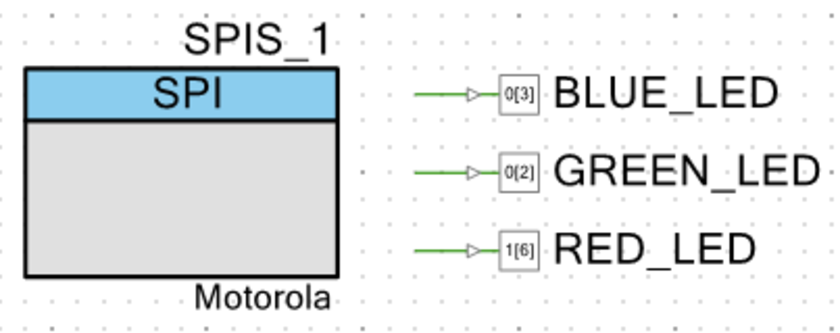
\includegraphics[width=0.4\textwidth]{filer/implementering/spi/spi_handler_topdesign}}
\caption{Topdesign for SPI og led}
\label{lab:topdesign_spi}
\raggedright
\end{figure}

Basis indstillingerne for SPI blokken ses i figur \ref{lab:spi_basic_config}. Mode sættes til slave, og SCLK mode sættes til CPOL=0, CPHA=0.

\begin{figure}[H] \centering
{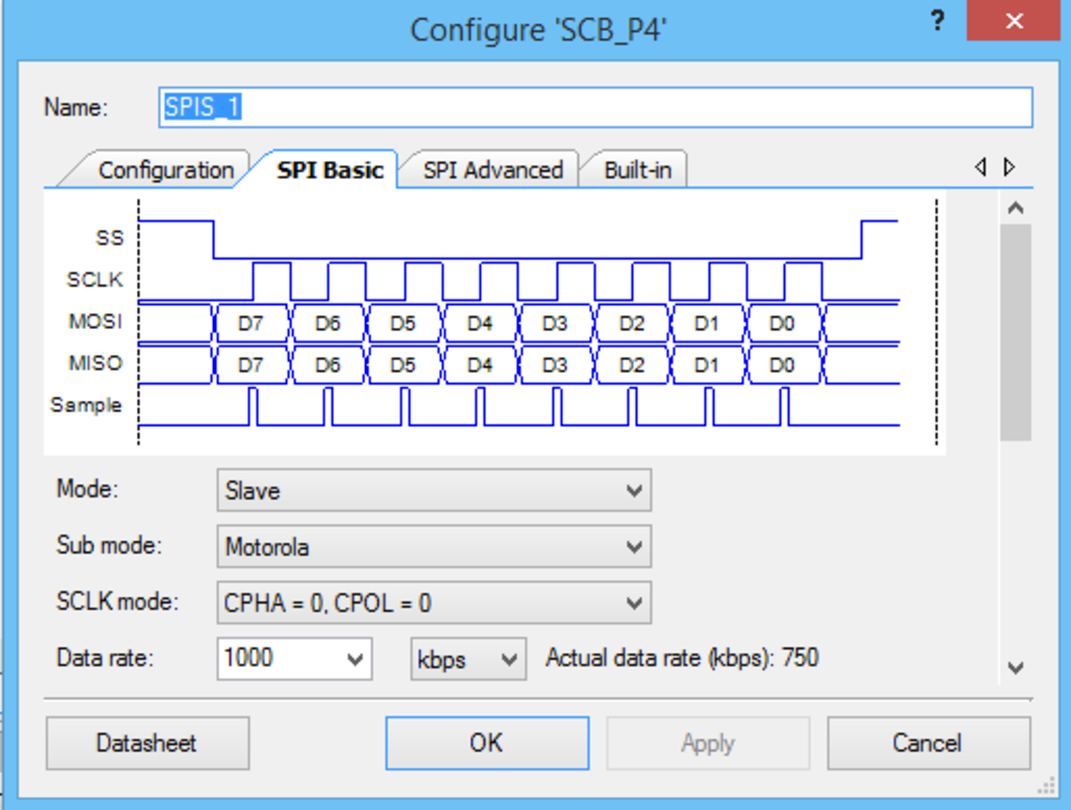
\includegraphics[width=0.7\textwidth]{filer/implementering/spi/spi_handler_topdesign_spi_basic}}
\caption{Konfigurering af SPI (SPI basic)}
\label{lab:spi_basic_config}
\raggedright
\end{figure}

De avancerede indstillinger for SPI blokken ses i figur \ref{lab:spi_advanced_config}. Buffer size sættes til 8 bit for både RX og TX. Interruptet sættes til internt og interrupt kilden er RX FIFO not empty og RX FIFO full.

\begin{figure}[H] \centering
{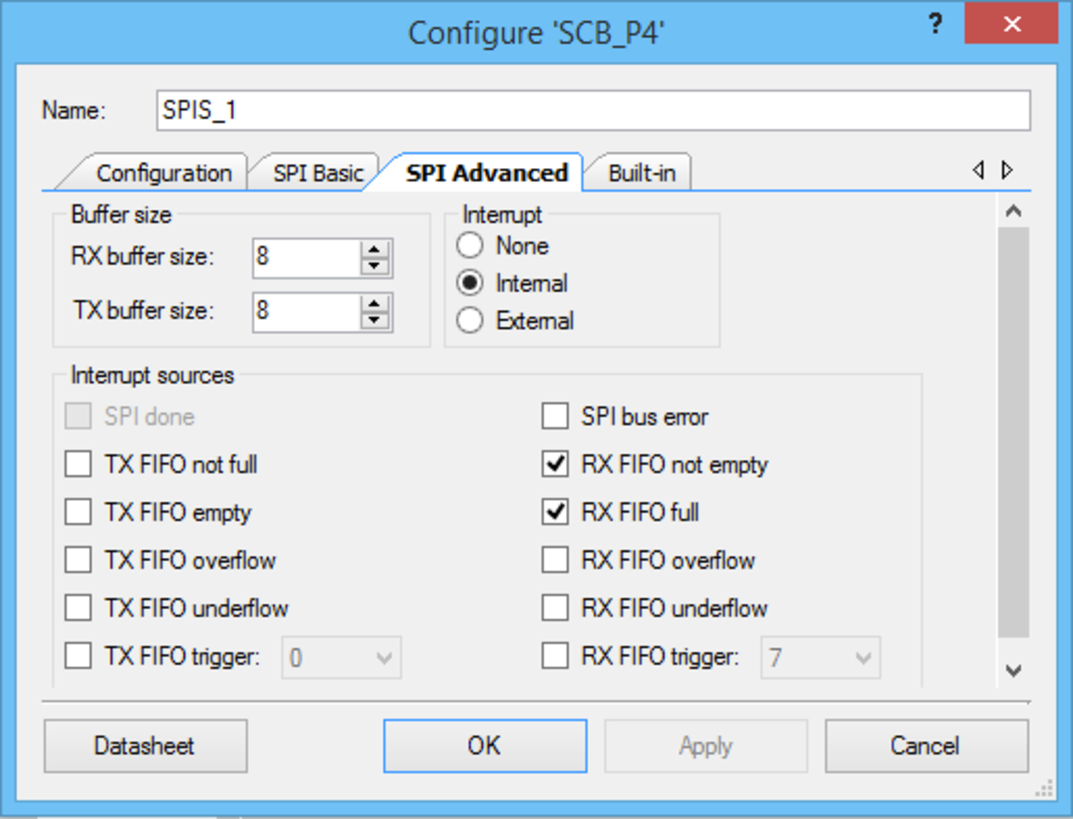
\includegraphics[width=0.7\textwidth]{filer/implementering/spi/spi_handler_topdesign_spi_advanced}}
\caption{Konfigurering af SPI (SPI advanced)}
\label{lab:spi_advanced_config}
\raggedright
\end{figure}

De 3 output pins (GREEN\_LED, BLUE\_LED, RED\_LED) skal sættes til digital output uden hardware connection.
Figur \ref{lab:led_pins_config} viser hvordan indstillingen skal være, dette er gældende for alle 3 pins. 

\begin{figure}[H] \centering
{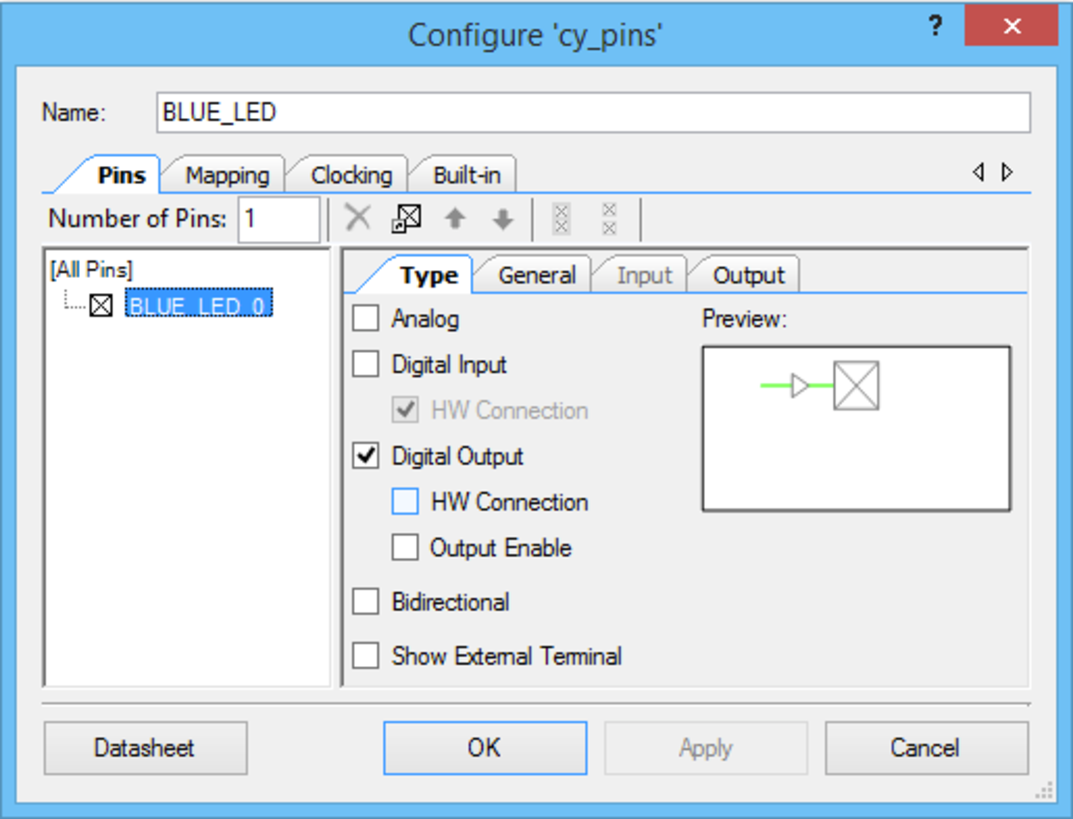
\includegraphics[width=0.7\textwidth]{filer/implementering/spi/spi_handler_topdesign_led}}
\caption{Konfigurering af pins}
\label{lab:led_pins_config}
\raggedright
\end{figure}


\subsubsection*{ISR}

SPI handleren består stort set kun af én interrupt rutine. Der tages udgangspunkt i de vigtige dele af rutinen. Og resten af koden kan ses i bilag.

Selve interrupt-rutinen er bygget op med en switch, der vælger en case alt efter input fra Masteren. Der tilgås kun switchen hvis der kommer en kommando der skal svare tilbage til Master (\verb+'R','L','V'+) eller en Clear buffer kommando \verb+'C'+, derefter kigges der på plads [0] i spiBuffer arrayet, og handles alt efter hvad der står der. Dvs. hvis Enheden skal aktiveres, sendes først et \verb+'A'+ fra Master som læses ind i spiBuffer[] arrayet efterfulgt af et \verb+'C'+ som tilgår switchen.
 
\begin{lstlisting}[language=C]
char spiBuffer[64];
..
..
..
CY_ISR(isr_spi_rx) {

	char cmd = '0';
	..
	.. 
	cmd = SPIS_1_SpiUartReadRxData();  
	spiBuffer[spiCounter] = cmd;
	spiCounter++;
	..
	..
	if ((cmd == 'R') || (cmd == 'C') || (cmd == 'L') || (cmd == 'V')){
	switch (spiBuffer[0]) {
	..
	..
\end{lstlisting}

Alle kommandoer der kræver et svar tilbage på SPI, bruger \verb+'R'+ casen, men eftersom PSoC4 kræver noget tid\footnote{HAL Exercise 7: Oplyses det at PSoC4 kræver 50us, men dette er ikke et problem da der laves én læsning ad gangen og der er min. 300ms i mellem hver læsning} til at hente og skrive i tx-bufferen er koden lavet sådan at man er på forkant med en læsning. Dvs. når der laves en læsning \verb+'R'+ fra Masteren, er der allerede skrevet til tx-bufferen, så man reelt læser data ud med det samme. 

Det er derfor switchen tilgåes ved alle ''Read'' kommandoer, så hvor der f.eks. skal verificeres, laves der en læsning af Enhedens enhedsnummer. I eksemplet nedenfor er en global char brugt som enhedsnummer, denne læses ind i tx-bufferen når case \verb+'V'+ køres. Når så case \verb+'R'+ køres, læses unitNo variablen først, hvorefter der skrives en ny værdi ind i tx-bufferen til næste \verb+'R'+ køres.


\begin{lstlisting}[language=C]
char unitNo = '1';
int spiCounter = 0;
int spiReadCounter = 0;
..
..
..
CY_ISR(isr_spi_rx) {
	..
	..
	..
	case 'V':
		..
		..
		..
		SPIS_1_SpiUartClearTxBuffer();
		SPIS_1_SpiUartWriteTxData(unitNo);
		spiCounter = 0;
	break;
	..
	..
	..
	case 'R':
		SPIS_1_SpiUartClearTxBuffer();
		SPIS_1_SpiUartWriteTxData(spiTxBuffer[spiReadCounter]);
		spiCounter = 0;
		spiReadCounter++;
	break;
\end{lstlisting}